\subsection{Fission of Induction State}
\label{sec:fission}


\begin{figure*}[t!]
\centering
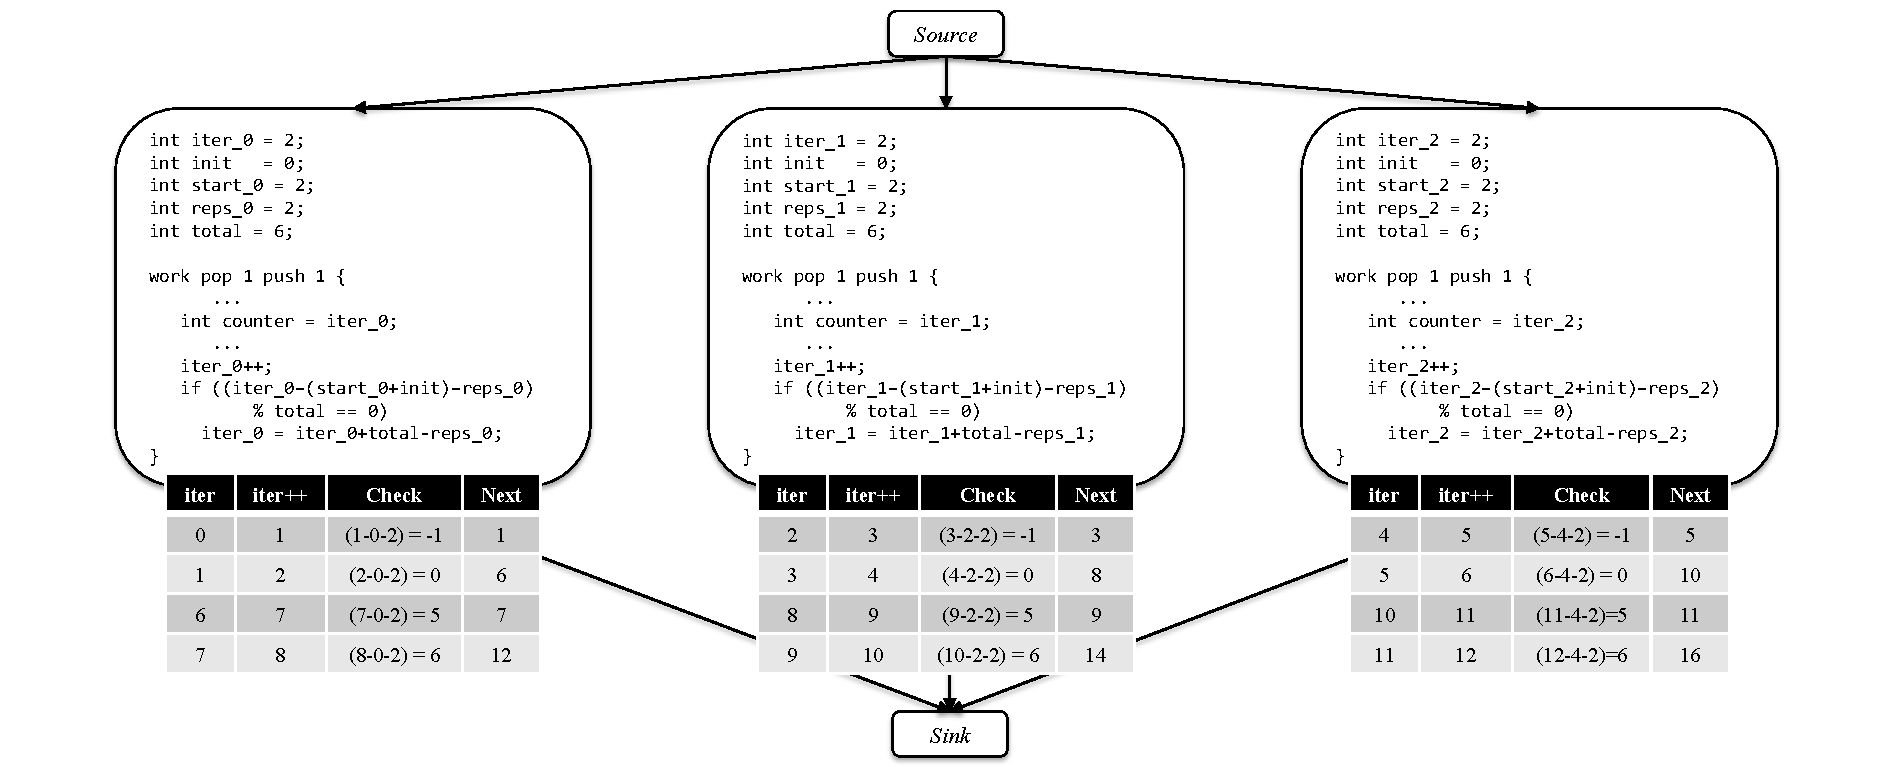
\includegraphics[width=6.5in]{figures/fission-example.pdf}
\caption{Example of an iteration filter fissed into three fission products each with multiplicity 2.  The chart indicates the values used to determine the next value of the iteration field.  \protect\label{fig:fission-example}}
\end{figure*}

The compiler introduces data parallelism to the streaming program through a process known as {\it fission}.  Fission is the process of duplicating the stateless filter and wrapping these duplicates in a round-robin splitter and joiner.  The process ensures that input data is distributed correctly and output data is collected in correct order.  The duplicated filters, known as products, can be assigned to individual cores, thus introducing data parallelism.  

Fission is applicable only to stateless filters, as the duplication process does not guarantee consistent behavior if filters contain state that changes between iterations.  Because the desugared iteration filters actually use mutable state to keep track of iteration values, the fission process must be modified to handle iteration values.  

\subsubsection{Modifications to Fission Process}

Let $F$ be the stateless filter that will be fissed.  Assume the fission process yields $N$ fissed products.  Accordingly, this yields the fissed products $F_0$, $F_1$, ... , $F_i$, ... , $F_{N-1}$.  The notation $F_{i}$ represents the $(i+1)$th fissed product of filter $F$.

The fission process now modifies the fission products by adding the
following values as fields to the products:
\begin{itemize}
    \item \texttt{init}: the multiplicity of the initialization schedule.  This value is determined for $F$ and is constant for all fissed products.
    \item $\texttt{reps}_i$: how often the \texttt{work} function of the product $F_i$ is
      invoked between rounds.
    \item $\texttt{start}_i$: the value of the induction variable each product $F_i$ starts with, less the initialization multiplicity.  Alternatively, $\sum_{j=0}^{i-1}{\tt reps}_j$ of all fission products preceding the current product.
    \item \texttt{total}: the periodic multiplicity of $F$.  Alternatively $\sum_{j=0}^{N-1}{\tt reps}_j$. This value is the same for all fissed products.
\end{itemize}
As described in ~\ref{sec:compiler-overview}, initialization execution is required for peeking filters to ensure every firing of the periodic steady-state schedule maintains the same number of leftover items on the channel.  This initialization execution of the original filter is transferred entirely to the first fission product.  However, all fission products must take the multiplicity of the initialization schedule into account in their calculations as the multiplicity is adjusted upwards by this value.

Accordingly, the fission product $F_i$ should start each round with iteration values of
\begin{eqnarray*}
\texttt{total}*\texttt{k} + (\texttt{start}_i + \texttt{init})
\end{eqnarray*}
and range up to the value
\begin{eqnarray*}
\texttt{total}*\texttt{k} + (\texttt{start}_i + \texttt{init}) + \texttt{reps}_i - 1
\end{eqnarray*}
where \texttt{k} is a nonnegative integer indicating how many rounds have
been run in the span of the program.  

At the end of each fission product's \texttt{work}, a check must be made to see if it is necessary to increment the induction variable to the next round of values.  This will prevent certain fissed products from making calls with duplicate iteration values.  This check is done after the field incrementing statement.
\begin{eqnarray*}
(\texttt{iter}_{i,k} - (\texttt{start}_i + \texttt{init}) - \texttt{reps}_i) \% \texttt{total} &==& 0
\end{eqnarray*}
This is consistent with the maximum value per round as
indicated above.  Only when we reach this maximum value does subtracting 
$\texttt{start}_i$, \texttt{init}, and $\texttt{reps}_i$ from $\texttt{iter}_i$ leave a value divisible by
\texttt{total}.

Once the fissed product's iteration value has reached
this value, it must be set to:
\begin{eqnarray*}
\texttt{iter}_{i,k+1} &=& \texttt{iter}_{i,k} + (\texttt{total} - \texttt{reps}_i) \\
&=& \texttt{total}*\texttt{k} + (\texttt{start}_i + \texttt{init}) + \texttt{reps}_i \\
&&  \ \ +\ (\texttt{total} - \texttt{reps}_i) \\
&=& \texttt{total}*(\texttt{k+1}) + (\texttt{start}_i + \texttt{init})
\end{eqnarray*}
which is the starting iteration value of the next round, as defined.

\subsubsection{Accounting for Steady-state Schedule Modification}

Other passes may modify the steady-state schedule after fission, increasing the multiplicity of the fission products.  This scales the $\texttt{reps}_i$ field for all products.  $\texttt{start}_i$ and $\texttt{total}_i$ are dependent on $\texttt{reps}_i$ and must be scaled accordingly.

Assume a pass increases hte steady-state multiplicity of our filter to $m$.  We expect the fission product $F_i$ to start round $k$ with iteration values of 
\begin{eqnarray*}
(\texttt{total}*\texttt{k}*m) + (\texttt{start}_i*m + \texttt{init})
\end{eqnarray*}
The filter should perform $\texttt{reps}_i$*$m$ iterations, thus should range up to value
\begin{eqnarray*}
(\texttt{total}*\texttt{k}*m) + (\texttt{start}_i*m + \texttt{init}) + (\texttt{reps}_i*m) - 1
\end{eqnarray*}

Between rounds, iteration values must be incremented by the actual total number of repetitions that occur.  All fission products perform a total of $\sum(\texttt{reps}_{i}*m)$ repetitions which is simply \texttt{total}*$m$.  Thus, the updating step will still hold:
\begin{eqnarray*}
\texttt{iter}_{i,k+1} &=& \texttt{iter}_{i,k} + (\texttt{total}*m - \texttt{reps}_i*m) \\
&=& \texttt{total}*\texttt{k}*m + (\texttt{start}_i*m + \texttt{init}) + \texttt{reps}_i*m \\
&&  \ \ +\ (\texttt{total}*m - \texttt{reps}_i*m) \\
&=& \texttt{total}*(\texttt{k+1})*m + (\texttt{start}_i*m + \texttt{init})
\end{eqnarray*}
